%SourceDoc ../YourName-Dissertation.tex
\vspace*{-80mm}
\chapter{Introduction} \label{chapter1:introduction}

For the past several decades, the primary focus in nuclear engineering
within the United States has been focused on light water reactors (LWR).
Commercially, all nuclear reactors are either boiling water reactors (BWR)
or pressurized water reactors (PWR). Correct computation of the
thermal hydraulics within the reactor core leads to efficient design and
accuracy in the safety analysis. A
popular subchannel code for modelling the hydrodynamics with in the reactor core is COBRA-TF.
This FORTRAN based code solves 8 conservation equations for liquid,
entrained droplet, and vapor phases in 3-D dimmensions \cite{CTF_Theory}.
The conservation equations analytically reduce into a pressure matrix in a
semi-implicit  method with rod temperatures solved for explicitly. Because
the physics are integrated into the numerical solution, the equations must
be linear and the solution method semi-implicit. With a residual
formulation, greater flexibility and control over the numerical solution
is possible. COBRA-TF was originally written in FORTRAN 77, but over
the years has been partially updated to newer versions of Fortran.

\begin{figure}[!h]
	\centering
	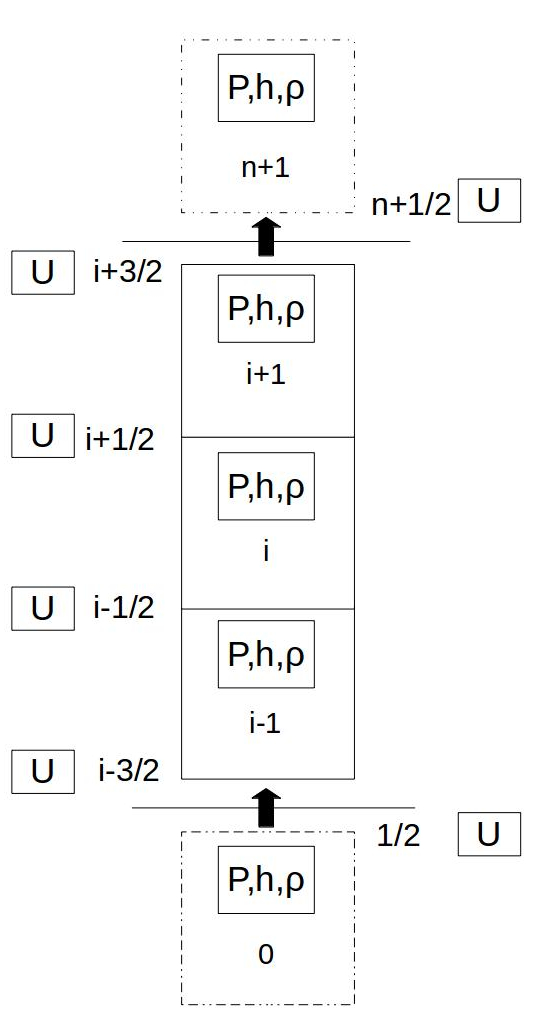
\includegraphics[width=0.30\textwidth]{images/CTF-Cells}
	
	\caption{The finite volume structure for COBRA-TF}
	\label{fig:CTF-Cells}
\end{figure}

The finite volume structure in COBRA-TF in figure \ref{fig:CTF-Cells} is for
a one-dimmensional channel in the axial direction with $n$ number of cells.
The first and last cells at $0$ and $n+1$ are ghost cells and act as the
boundary conditions for the problem. Pressure, enthalpy, and density are
averaged over the cell volume and are located at the center of the cell.
Mass flow rate and velocity are located at the faces in between cells. The
cells are represented with an index $i$, and the faces with indexes of
$i+\frac{1}{2}$ or $i-\frac{1}{2}$. This project will initially focus
on this 1-D configuration. Usually the code is three dimensional, with
channels connecting to each other in two more dimmensions. Fully 3-D
equations will be considered in future work.

\section{Background}



